%!TEX root = ../dissertation.tex

\chapter{Origins of a complexity bias}
\label{chapter:origins}

\section{Introduction}

A universal property of languages is that they contain units of meaningful sounds---words---that vary in length. What accounts for this variability? That is, why is the word for ``can'' short but the word for ``calculator'' long? One class of explanations for this variability appeals to properties of the linguistic form itself, such as word frequency \cite{zipf1936} and predictability in linguistic context \cite{piantadosi2011a,mahowald2013info}. Our recent work has revealed an additional factor influencing word length: conceptual complexity. Across 80 natural languages, we find a bias for longer words to refer to conceptually more complex meanings \cite<a {\it complexity bias};>{lewisstructure2014}. This systematicity between word length and meaning challenges the long-held assumption that the relationship between form and meaning is entirely arbitrary \cite{saussure}. 


%%%MCF
%What is the source of this bias, and how could a complexity bias affect the lexicons of a diverse set of languages? We first briefly consider the source of such a bias, and then we turn to the topic of the current paper: the mechanism by which a complexity bias could influence language change.
%
%While many explanations of the complexity bias are possible, we consider two here. First, a complexity bias could reflect a general cognitive bias for similarity. This account suggests that longer words get mapped to more complex referents because they both share the abstract quality of complexity. This proposal is consistent with other instances of iconicity in natural language \cite<see>[for review]{schmidtke2014phonological}. Second, perhaps a complexity bias emerges from principles of communication. As part of a broader theory of communication, \citeA{horn1984} suggested that a contrast in length between two phrases with the same denotational value implies a contrast in meaning, with the longer phrase getting the more unusual or complex meaning. 
%
%Thus, the complexity bias observed in the lexicon could reflect this in-the-moment communicative bias---an appealing possibility given evidence that other features of the lexicon also reflect principles of communication, like the structure of semantic space \cite{regier2007color, kemp2012kinship, piantadosi2012communicative}.
%
%Both the similarity and communicative accounts posit pressures on the lexicon that take places across multiple timescales. They suggest that speakers have a complexity bias that is psychologically real in the moment of language use and that this bias emerges in the structure of the lexicon over the course of language evolution. These hypotheses make the critical prediction that we should be able to observe this bias not only in the structure of natural languages, but also in one-shot learning tasks with novel words. In previous work, we have found robust support for this prediction. Across a range of stimuli, and both comprehension and production tasks, we find that speakers are biased to map a longer novel word onto a more complex novel referent, relative to a shorter word \cite{lewisstructure2014}.
%
%But for the complexity bias to be present in the lexicons of natural languages suggests that it must affect language change. How does an in-the-moment complexity bias leads to a regularity in the lexicon over time? We propose that this bias causes small changes in memory for complex phonological forms, leading to biases in linguistic transmission across generations that result in a lexicon that magnifies these small biases \cite{griffiths2007language}. In the present work, we begin to test this hypothesis using the iterated learning paradigm, a recently-developed method for studying language change in the lab \cite<e.g.,>{kirby2008cumulative, reali2009evolution, smith2010eliminating}. The critical feature of this paradigm is that the learning output of one speaker becomes the learning input for a new speaker. This paradigm allows us to examine the evolution of a language for a ``chain'' of speakers learning and transmitting a language. The dynamics of these chains serve as an approximation of the dynamics of generations of children acquiring and then transmitting language to future generations. 



% latex table generated in R 3.1.0 by xtable 1.7-4 package
% Fri Jan 23 11:41:41 2015
\begin{table*}[t]
 \footnotesize
\centering
%\begin{tabular}{r|llllllllll}
%\begin{tabular}{r| |l | l |l |l |l|l |l |l|l| l}
\begin{tabular}{c rrrrrrrrrr}
\hline
 \multicolumn{11}{c}{Object} \\
 \hline

 \rule{0pt}{2ex}    
& 1 (Q1) & 2 (Q1) & 3 (Q2) & 4 (Q2) & 5 (Q3) & 6 (Q3) & 7 (Q4) & 8 (Q4) & 9(Q5) & 10 (Q5) \\ 
 \hline
    {\it Gen.\ 0} & damitobup & nagir & nid & gimunobugup & dunobax & mikupudax & bipag & daganitobip & nimimog & gan \\ 
   {\it Gen.\ 1}& nilobup & niger & nid & runtunbug & dunobug & bipoxtog & bipag & dipentag & nimimog & gan \\ 
    {\it Gen.\ 2} & nilobup & niger & nid & runtunbug & dunbug & ripenbog & bippenbog & dipentag & nimobop & gan \\ 
  {\it Gen.\ 3} & nilobop & niger & nid & rittenbob & dabop & rudentag & buttenbug & dertag & nimobop & gar \\ 
   {\it Gen.\ 4} & nilobop & niger & nid & bittenbob & dabop & rittenbog & buttenbop & dertag & nimbobop & gar \\ 
    {\it Gen.\ 5}  & nilop & niger & nir & girbop & dabop & dirbop & bittenbop & rittenbog & nilobop & dir \\ 
   {\it Gen.\ 6}& nilop & niger & nir & garbog & dabop & dabog & bittenbop & rittenbog & nilop & dir \\
   {\it Gen.\ 7}& nilop & niger & hir & garbop & dabog & dabog & bittenbop & rottenbog & nilop & dir \\ 
\hline
\end{tabular}
\caption{A representative language chain. Words are presented for each of the 10 objects across 7 generations and the initial input language. The complexity quintile of the object is noted parenthetically. Across generations, words tend to get shorter, less unique, and phonotactically more probable. Words also become more likely to be remembered accurately.}
\label{tab:ex}
\end{table*}
\normalsize



%%%MLL

The origins of this bias  in language are an open question. One possibility is that the bias is due to a pressure in individuals to map longer words onto more complex meanings. Under this account, there is a psychological bias to map longer words onto more complex meanings---a synchronic complexity bias---and over time this bias leads to this same regularity emerging in the structure of the lexicon---a diachronic complexity bias. In the present paper, we consider the mechanism through which a synchronic complexity bias in individuals might lead to diachronic change in the lexicon.  

There are several possible sources for a psychological, synchronic complexity bias. For example, the bias could reflect a more general cognitive preference for iconicity \cite<see>[for review]{schmidtke2014phonological}.  A second alternative is that the bias  is related to principles of communication.   As part of a broader theory of communication, \citeA{horn1984} suggested that a contrast in length between two phrases with the same denotational value implies a contrast in meaning, with the longer phrase getting the more unusual or complex meaning. Thus, the complexity bias  in the lexicon could reflect this in-the-moment communicative bias---an appealing possibility given evidence that other features of the lexicon also reflect principles of communication, like the structure of semantic space \cite{regier2007color,kemp2012kinship,piantadosi2012communicative}. 

Critically, if the emergent diachronic bias is due to a psychological synchronic pressure, we should be able to observe this bias not only in the structure of natural languages, but also in one-shot learning tasks with novel words. In previous work, we have found robust support for this prediction. 
 Across a range of stimuli, and both comprehension and production tasks, we find that speakers are biased to map a longer novel word onto a more complex novel referent, relative to a shorter word \cite{lewisstructure2014}.
 
How does a synchronic complexity bias lead to diachronic change in the lexicon? The causal mechanism for this type of change would have to take place over multiple timescales: A synchronic bias in the moment of language interaction would have lead to changes in the lexicon over the course of language evolution. We propose that a psychological bias causes small changes in memory for complex phonological forms in the moment of language interaction, and  this  pressure leads to biases in linguistic transmission across generations. Over the course of language evolution, these psychological, synchronic biases result in a lexicon that magnifies these biases  \cite{griffiths2007language}. 

In the present work, we begin to test this hypothesis using the iterated learning paradigm, a recently-developed method for studying language change in the lab \cite<e.g.,>{kirby2008cumulative,reali2009evolution,smith2010eliminating}. The critical feature of this paradigm is that the learning output of one speaker becomes the learning input for a new speaker. This paradigm allows us to examine the evolution of a language for a ``chain'' of speakers learning and transmitting a language. The dynamics of these chains serve as an approximation of the dynamics of generations of children acquiring and then transmitting language to future generations. 

A secondary goal of the present work is to examine how psychological pressures influence the structure of the lexicon, independent of conceptual pressures.  Forms that are difficult to remember are unlikely to survive in the language  \cite{christiansen2008}, and there may be an additional communicative pressure for economy of expression \cite{zipf1949human}. Both of these pressures might lead to a preference for shorter words over longer, harder-to-produce words, biasing the ultimate structure of the lexicon towards shorter, more memorable words. 
% The lexicon that emerges would then be an equilibrium state resulting from these multiple pressures.

% This proposed mechanism extends beyond the individual speaker; it relies on the diachronic emergence of the bias through the interaction of many individuals over the course of the language change timescale (i.e.\ many years). No existing data bears on this relationship, in part because the macro-level features of the hypothesis make it difficult to test empirically and, in particular, experimentally. 

%The goal of the present experiment is to explore the relationship between in-the-moment, psychological pressures on the lexicon and the effect of cumulative effect of these pressures over time.

We used an iterated learning paradigm to study the dynamics of these two aspects of the lexicon: how  words change over the course of language evolution and how conceptual complexity interacts with these changes.\footnote{For ease of measurement, we operationalize word length in terms of number of orthographic characters. However, this measure is highly correlated with measures of length with greater psychological reality, such as phonemes and morphemes \cite{lewisstructure2014}.} As predicted, we find that forms in the lexicon converge to a more stable state and that a complexity bias emerges in the mappings between words and referents. We also find, contra our hypothesis, that the complexity bias is attenuated over time. A post-hoc analysis suggests that this change in the complexity bias over time is related to the degree of cross-generational change in the lexicon.

% In particular, we in-the-moment complexity bias might influence the mappings that emerge between words and meanings over time. We used an artificial language iterated learning paradigm to explore these questions. We find that the lexicon converged to a more stable state, and that 

%hypothesized that without any conceptual pressures

%how a goal of the present experiment is to explore how features of the lexicon are influenced by the process, and how conceptual pressures interact with these pressures. 

% In order to examine a possible relationship between an in-the-moment complexity bias and a lexical complexity bias, A secondary goal was to explore first-order changes in the lexicon that emerge as a consequence of iterated learning. We find that a complexity bias emerges early in the evolution of the language, but contrary to the Emergence Hypothesis, is washed out by the pressure to simplify the language. In the General Discussion, we speculate this may be due to the non-communicative nature of the task. 

%* converged, and suggestive evidence
%* changes in the lexicon and effect of
%* first order converged to more stable 
%* we hypothesized without conceptual pressures 






%%%% EXPERIMENT 1 %%%%%%
\section{Experiment }

Given existing evidence that a complexity bias is present in one-shot learning games \cite{lewisstructure2014}, our experiment was designed to test how conceptual pressures influenced the lexicon over the course of transmission. We asked speakers to learn a novel language that contained meanings of varying complexity and words of varying length. Critically, the language we asked participants to learn contained no systematic relationship between complexity and word length. After studying these mappings, participants were asked to recall them. The measure of interest was the relationship between the errors participants made and the complexity of the referent. If participants show a complexity bias, they should be more likely to add characters for more complex objects and remove characters for less complex objects. 

This design characterized the first generation of our task. We then gave the labels that participants produced in the test phase of this first generation to a new set of speakers and asked them to complete the exact same task. We iterated 7 generations of this task in total.


\subsection{Method}

\subsubsection{Participants} 

We recruited 350 participants from Amazon Mechanical Turk. Each generation was composed of 50 learners.

\subsubsection{Stimuli}

The referents were a set of 60 real objects that did not have common labels associated with them. These objects had been normed for their complexity in previous work \cite[Figure\ 1]{lewisstructure2014}. Norms were obtained by asking participants to indicate ``How complicated is this object?" using a slider scale. Norms were highly reliable across two samples of 60 participants. Based on these norms, we divided the objects into quintiles of 12 objects each. Each participant saw 2 objects from each quintile. 
%\squeezeup

\begin{figure}[b!]
\begin{center}
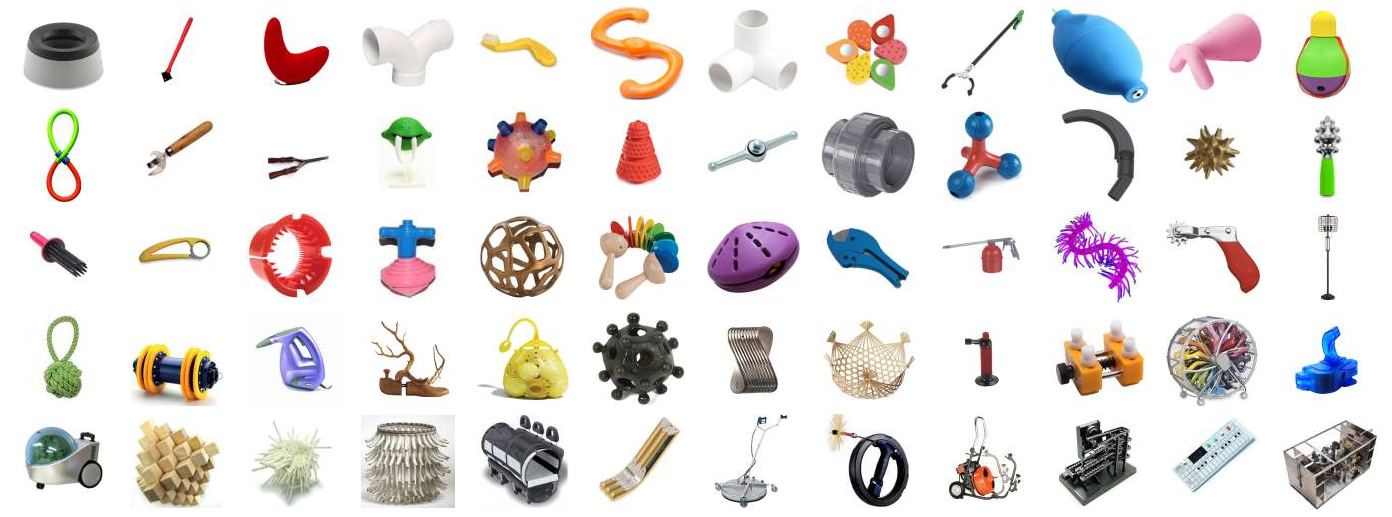
\includegraphics[width = 1\linewidth]{figs/realobjs.pdf}
\end{center}
\vspace{-.24em}
\caption{Object stimuli used in the Experiment. The objects are sorted from least complex (top left) to most complex (bottom right) based on the complexity norms in Lewis et al.\ (2014). Each row corresponds to a quintile.}
\label{fig:objs}
\vspace{-1em}
\end{figure}


\begin{figure*}[t]
\begin{center}
\includegraphics[scale = .35]{figs/Plot1.pdf}
\end{center}
\vspace{-.5em}
\caption{Changes in lexical features across generations. Error bars represent 95\% confidence intervals computed via non-parametric bootstrap across chains.}
\label{fig:length}
\vspace{-1em}
\end{figure*}

In the first generation, the words were composed of randomly concatenated syllables of 3, 5, 7, 9 or 11 characters in length. Words contained CV syllables and ended in a consonant (e.g., ``gan," ``panur," ``pugimog," ``tigadogog," and ``mogonokigan"). Each participant saw 2 words of each length. The assignment of word lengths to objects was arbitrary.

Participants in Generation 2 were yoked with a participant from this first generation. This meant a participant in Generation 2 would see the exact same set of pictures as the yoked participant from Generation 1, but would learn the labels for those objects that the yoked participant had produced in the testing phase of Generation 1. Order of presentation in the training phase was randomized across generations. We iterated this procedure for a total of 7 generations.

\subsubsection{Procedure} 


Participants viewed a webpage that informed them they would be learning the names of 10 objects in an alien language. They were told they would see the names for each object four times and then their memory for the name of each object would be tested. Participants next viewed a screen displaying an object and the associated label below it. Participants pressed the space bar to advance to the next picture. Each picture-word pair was shown four times. 

In the test phase, participants saw a screen with a picture and were asked to type the learned label in a text box below the picture. Memory for each of the 10 objects was tested.





\subsection{Results}



We conducted three analyses exploring how iterated learning influenced the structure of lexicons.\footnote{All code and data for the paper are available at \url{http://github.com/mllewis/iteratedRC}.} In Analysis \#1, we examined the evolution of lexical forms. In Analysis \#2, we considered the relationship between word length and referent complexity. This was the key analysis because it allowed us to test for a complexity bias in the lexicon and how this bias changed over time. Finally, in Analysis \#3, we conducted a post-hoc analysis to understand the source of variability in cross-generational change in complexity bias across chains.

\begin{figure}[t]
\begin{center}
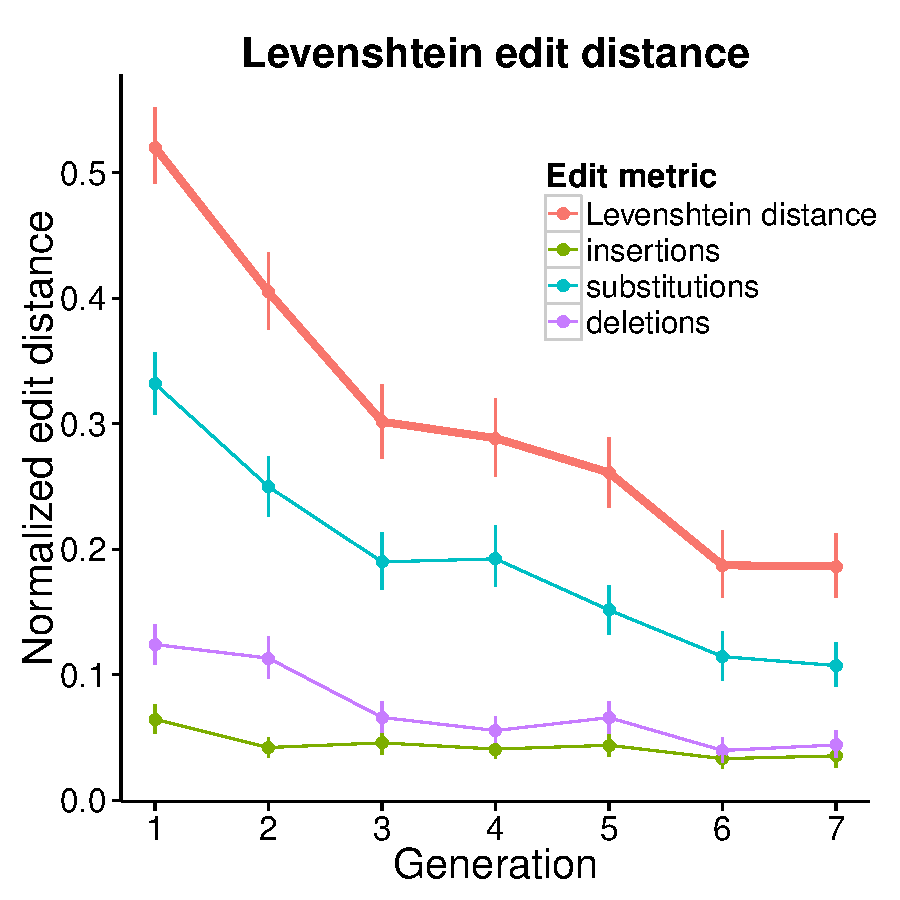
\includegraphics[width = .7\linewidth]{figs/lev.pdf}
\end{center}
\vspace{-.5em}
\caption{Edit distance across generations, normalized by length of the longest word (guessed word vs.\ actual word). The top line shows the Levenshtein edit distance. The lines below reflect the components of this metric (substitutions, deletions, and insertions). Error bars represent 95\% confidence intervals computed via non-parametric bootstrap across chains. Number of edits decreased across generations.}
\label{fig:lev}
\vspace{-1em}
\end{figure}

\begin{figure*}[t]
\begin{center}
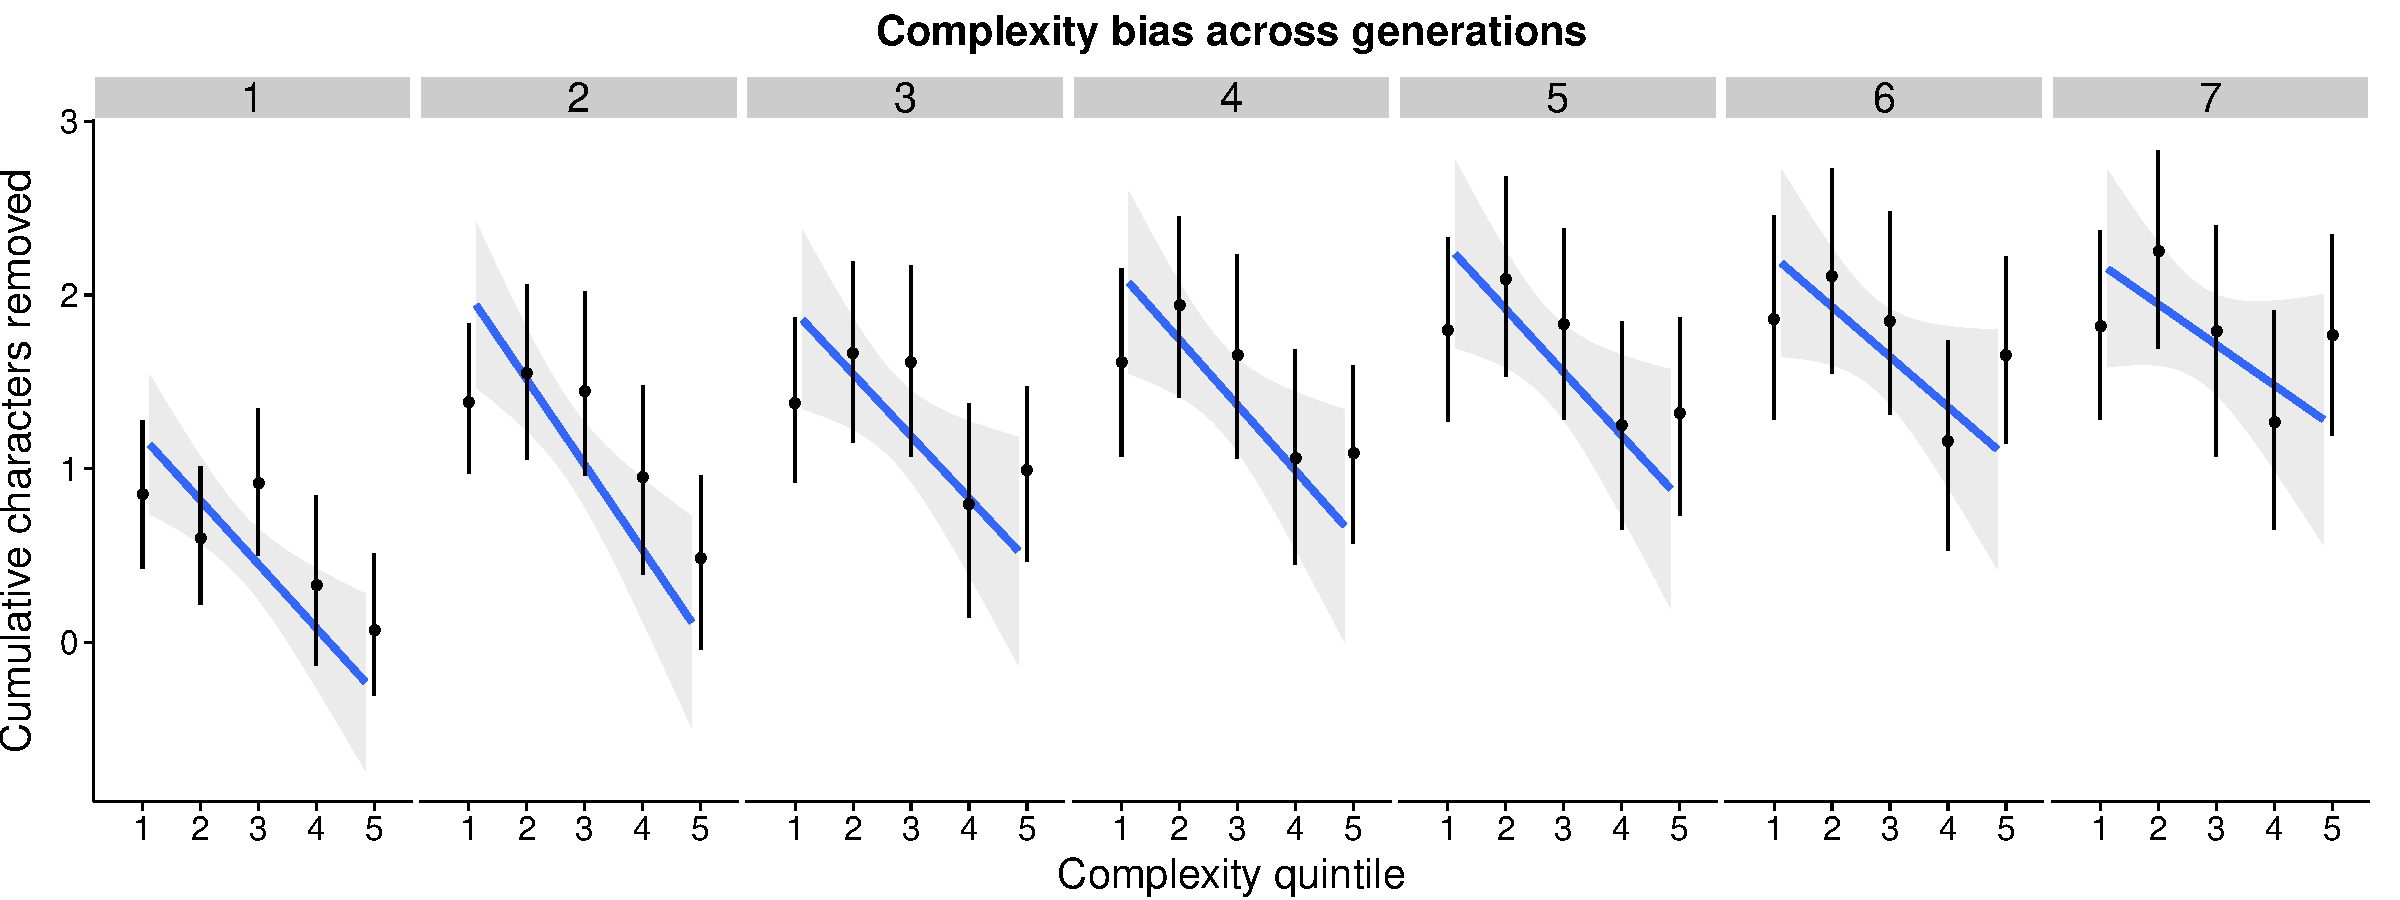
\includegraphics[scale = .4]{figs/complexity_bias.pdf}
\end{center}
\vspace{-.5em}

\caption{Cumulative characters removed as a function of complexity across all 7 generations. Points correspond to the quintile means. Lines represent the best fitting linear model predicting word length from the complexity norm of the object. Negative slopes indicate a bias to recall longer labels for  more complex objects. Across generations, this bias decreased.}
\label{fig:cbias}
\vspace{-1em}
\end{figure*}

Across generations, 1\% of object labels were excluded because they contained more than one word or no word was produced. In these cases, the object was re-assigned a label from a different participant in that generation. The label was selected from a trial that had both the same initial word length and an object from the same quintile. 

\subsubsection{Analysis \#1: Word forms}


Table \ref{tab:ex} presents a representative language chain. We analyzed four features of the lexical forms, averaging across each of the 50 chains at each generation: mean word length, number of unique words, transition probability, and accuracy. We also analyzed the degree of lexical change at each generation using the Levenshtein edit distance metric.

Across generations, mean word length decreased from an initial length of 7 characters to 5.22 characters in Generation 7 ($SD= 2.25$; $r=-0.22, p<.0001$; Figure\ \ref{fig:length}a). The number of unique words also decreased across generations ($r=-0.35, p<.0001$; Figure\ \ref{fig:length}b). Lexicons tended to reduce in size by mapping the same word to multiple objects (e.g.,\ in the chain presented in Table \ref{tab:ex}, ``nilop'' refers to both Objects 1 and 9).



Third, the mean orthographic transition probability of each word increased across generations ($r=.52, p<.0001$; Figure\ \ref{fig:length}c). Transition probabilities were calculated based on the set of words in the lexicon for a particular participant at a particular generation. This finding suggests that lexicons became more phonotactically structured across time. We also calculated the mean transition probability of each word using English transitions. Probabilities were estimated via orthographic bigrams from the Google Books corpus \cite{norvig}. In this analysis, the mean English transition probability of each word also increased across generations ($r=0.18$, $p <.001$), suggesting that the orthographic structure of individual words became somewhat more similar to English across generations. % vowel/consonants


Fourth, we found that participants became more accurate in recall across generations ($r=.46, p<.0001$; Figure\ \ref{fig:length}d). To examine the relationship between accuracy and word forms, we constructed a logistic mixed-effects model predicting accuracy with word length, word uniqueness, and transition probability.\footnote{The model specification was as follows: \texttt{accuracy $\sim$ guessed label length~$\times$~transition probability~$\times$~ uniqueness + (guessed label length~\textbar~subject) +  (1~\textbar~chain)}.} Only word length was a reliable predictor of accuracy ($\beta=1.21$, $p <.0001$), suggesting that perhaps the increase in accuracy across generations was due to the shorter length of the words in these languages. %phonotactics is highly collinear with number of unique words so can't put in both predictors [f


%To examine the relationship between accuracy and features of the lexical forms, we constructed an additive linear model predicting accuracy with word length, number of unique words, and mean bigram probability. Both word length ($\beta=-0.25$, $p <.0001$) and number of unique words ($\beta=-0.28$, $p <.0001$) were reliable predictors of accuracy. This suggests that the increase in accuracy across generations was related to these changes in the features of the lexicon.

Finally, we analyzed word changes across generations using Levenshtein edit distance. This measure provides a formal metric of the similarity between two strings. Levenshtein edit distance is computed by counting the minimum number of character edits necessary to transform one word into another. For example, the edit distance from ``can" to ``cat" is 1 (1 substitution), while the edit distance from ``can" to ``calculator" is 8 (1 substitution and 7 insertions). For each word, we calculated a normalized measure by dividing the edit distance between the guessed word and the actual word by the length of the longest of the two. This normalized measure controlled for the decrease in word length across generations.  Across generations, the normalized edit distance decreased ($r=-.30, p<.0001$; Figure\ \ref{fig:lev}). This decreasing trend also held for each of the components of the Levenshtein metric: number of deletions ($r=-.18, p<.0001$), insertions ($r=-.08, p<.0001$) and substitutions ($r=-.27, p<.0001$). 

Taken together, this set of analyses points to a lexicon that is evolving to become more regular and consequently easier to learn.



                         


%consonant/vowel analysis?

\subsubsection{Analysis \#2: Complexity bias} 

In Analysis \#2, we examined the relationship between changes in word length and the complexity of referents. If there is a complexity bias in the lexicon, participants should be more likely to produce longer labels for more complex referents. 

We considered two metrics of word length: Label length in characters and cumulative characters removed (CCR). CCR is calculated by subtracting the word length at a particular generation from the input generation word length. Though slightly more complex, CCR provides a length metric that controls for variability in input word length; this control is important because words varied dramatically in their initial length due to random assignment in the initial generation. We calculated $p$-values based on an empirical distribution of $r$-values, obtained by sampling from random pairings of words and objects. This was done because changes in  language forms across generations change the distribution of possible $r$-values.

Across generations, there was a reliable bias to map longer words to more complex referents across both measures of length (label length: $r=.05, p<.05$; CCR: $r=-.11, p<.0001$). Figure \ref{fig:cbias} shows CCR as a function of object complexity across generations. Qualitatively, the bias decreased across generations. However, there was high variability across chains both in the total complexity bias (label length: $SD = .27$), and in how this bias changed across generations (label length: $M = .004$; $SD = .69$).

\begin{table}[t!]

\centering
\begin{tabular}{cc|ccccccc}

\multicolumn{2}{c}{\multirow{2}{*}{}} & \multicolumn{4}{c}{Quintile \#1}\\
\multicolumn{2}{c|}{}                    & 2 & 3 & 4 & 5\\ \cline{2-6}
\multirow{4}{*}{\rotatebox{90}{Quintile \#2}} & 1 & 86 &  78 & 64 & 52 \\
                                      & 2 &    &   84 & 63 & 34\\
                                      & 3 &   & & 41 & 59\\
                                       & 4 &   &  &  & 58\\
                                       \vspace{-.5em}

\end{tabular}  

\caption{Contingency table of trials where participants recalled the same word for multiple objects. Columns correspond to the complexity quintile of the target object and rows correspond to the  complexity quintile of the object with the same word. The diagonal is excluded because the experimental design restricted the number of possible confusions for these cases (1 possible alternative vs.\ 2 for all other quintiles). In cases of confusions, participants tended to reuse a word from an object in a nearby quintile.}
\label{tab:confusion}
\end{table}

A number of other exploratory analyses suggest a role for complexity in language change. First, Levenshtein edit distance was systematically related to the complexity of referents: Participants were more likely to edit words referring to more complex referents ($r=.05, p<.01$). Second, there was systematicity in the kinds of errors participants  made when reusing words across multiple objects. Participants tended to reuse labels from objects of nearby quintiles (Table\ \ref{tab:confusion}), suggesting that these labels were more conceptually confusable and lead to more category-formation.

Together, this set of analyses replicates prior work suggesting a complexity bias in the lexicon: Across both measures of word length, participants tended to recall longer labels to refer to more complex referents. They were also more likely to edit words related to more complex referents and reuse labels of objects from nearby quintiles. However, an unexpected finding was the attenuation of this bias across generations. In our last analysis, we try to understand this trend.

%\begin{figure}[t]
%\begin{center}
%\includegraphics[scale = .4]{figs/confusion.pdf}
%\end{center}
%\caption{Contingency table for all trials in which participants recalled the same word for multiple referents. The diagonal is excluded because the experimental design restricted the number of possible confusions for these cases (1 possible alternative vs.\ 2 for all other quintiles). When a participant mapped the same word to a second referent, they tended to reuse a word from an object in a nearby quintile.}
%\label{fig:confusion}
%\end{figure}
% latex table generated in R 3.1.0 by xtable 1.7-4 package
% Tue Feb  3 10:17:16 2015

   


\subsubsection{Analysis \#3: Relationship between change in word forms and change in complexity bias} 


We  conducted a post-hoc exploration of the variability in the complexity bias across chains. For each chain, we quantified the complexity bias at each generation by calculating the correlation between metrics of length (label length and CCR) and the complexity norms. We then calculated the correlation between these coefficients and generation. This gave us a measure of the change in the complexity bias across generations. We considered how this change in complexity bias related to the degree of change in the forms of the lexicon. Two metrics of lexical change were analyzed: accuracy and Levenshtein edit distance. 

Chains with greater cross-generational change in lexical forms tended to show an increase in complexity bias over time. Using raw label length as the length metric, there was a reliable correlation between change in complexity bias and accuracy ($r=0.29$, $p <.05$) and between  change in complexity bias  and normalized Levenshtein edit distance ($r=-0.32$, $p =.02$). This same pattern also held for the CCR length metric (accuracy: $r=-0.37$, $p <.01$; Levenshtein: $r=0.38$, $p <.01$; Figure\ \ref{fig:levcbias}).


\begin{figure}[t]
\begin{center}
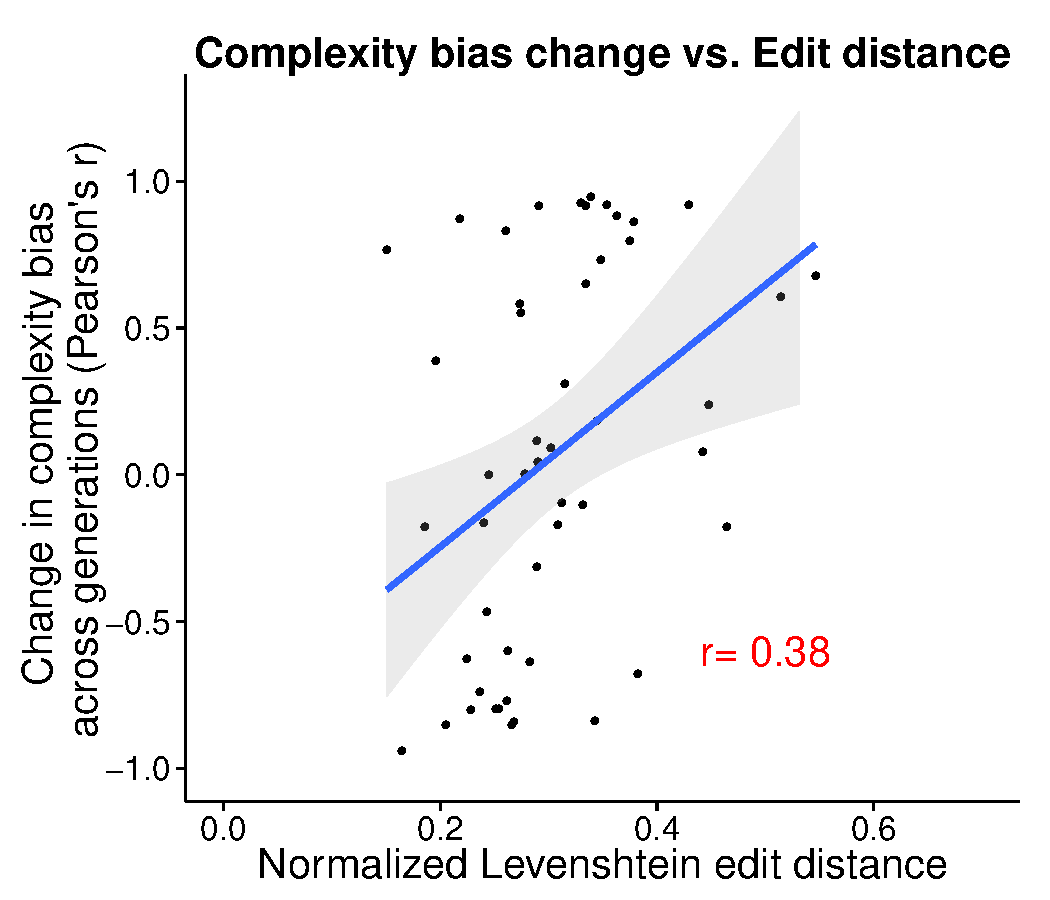
\includegraphics[width = .8\linewidth]{figs/change_plot.pdf}
\end{center}
\vspace{-.5em}
\caption{Complexity bias as a function of the normalized Levenshtein edit distance of the chain. Complexity bias is calculated here using number of cumulative characters removed. Each point corresponds to an individual chain. Chains with greater normalized Levenshtein distances tended to show a greater increase in complexity bias across generations.}
\vspace{-1.5em}
\label{fig:levcbias}
\end{figure}

%A negative coefficient indicated an increase in complexity bias over time, while a positive coefficient indicated a decrease in complexity bias over time. 

\subsection{Discussion}

In three analyses, we examined change in the structure of lexicons across generations of transmission. Analysis \#1 reveals that lexical forms become simpler and more regular over time. We find that words become shorter, less unique, more phonotactically probable, and more likely to be remembered. We also find that this structure facilities memory recall: lexicons with fewer and shorter words are more likely to be remembered accurately. Analysis \#2 examined the relationship between lexical forms and conceptual structure, and found that a complexity bias emerges in the lexicons. 

An unpredicted result was that the complexity bias does not strengthen across generations. Analysis \#3 suggests that change in the complexity bias across generations is related to the degree of change in lexical forms in the chain: Chains with more change are more likely to show an increase in complexity bias over time. The underlying mechanism supporting this relationship is straight-forward: chains that make more errors have more opportunity to deviate from the random input mappings between words and referents. This direction of this correlation suggests that when chains do in fact deviate from these initials mappings, they do so in a systematic way. That is, they tend to deviate in a way that is more likely to map longer words onto more complex referents.

%Nonetheless, there was great variability in the change in the complexity bias over time across each of the 50 chains. Analysis \#3 attempted to account for this variability. We find a correlation between the accuracy of the chain and the change in the complexity bias over time. In particular, we find that less accurate chains tend to show a larger complexity bias.
%%%% DISCUSSION %%%%%%
\section{General Discussion}

The iterated learning paradigm provides an opportunity to examine how in-the-moment psychological pressures influence the structure of a language in aggregate, over time. We examined two aspects of this structure: lexical forms and the mappings between words and objects. We hypothesized that different psychological pressures would influence each type of structure. In the case of lexical forms, we predicted there would be a bias to simplify the language into shorter, fewer forms. In the case word-object mappings, we predicted a bias to map longer words onto more complex meanings \cite{lewisstructure2014}. The question of interest was how these psychological pressures influenced the structure of the lexicon across generations of transmission. 

Our findings suggest that each of these pressures may have influenced the structure of the lexicon---and critically---that they interacted with each other. We found both a bias to simplify the lexicon and a bias to map longer words onto more complex meanings. But these pressures appear to have pushed in opposite directions: The pressure to simplify the language leads to less variability in word length, and this reduced variability suppresses the complexity bias. 

%We speculate, therefore, that a strong pressure to simplify the language may have lead to the attenuation of the complexity bias across time. In addition, simplifying the language may have lead to greater accuracy in transmitting the language, and this greater accuracy may have reduced the opportunity for a complexity bias to emerge. This interpretation is consistent with our post-hoc analysis demonstrating that less accurate chains showed a greater increase in complexity bias. 

If these dynamics reflect actual language evolution, however, an important question still remains---why do we in fact see a complexity bias in natural language? That is, if there is a strong pressure towards simplicity, then why does a complexity bias emerge in natural language despite this pressure? 

One possibility is that this discrepancy is due to the absence of an important feature in our task: communication with a second interlocutor. \citeA{zipf1949human} argued that the equilibrium that emerges in the lexicon is a product of both the speaker's desire to say less and the listener's desire for a more explicit, comprehensible message. Importantly, the common desire for efficiency creates opposing pressures among interlocutors. For a speaker, the optimal solution to communication is to have a lexicon that contains a single, short word that can be used to refer to all meanings. However, for a listener, the optimal solution is to have a lexicon that maps a unique word onto every possible meaning. 

Thus, perhaps the absence of a listener pressure in our task may have lead our participants (``speakers'') to simplify the language. While our task was posed as a memory task, there was no penalty for failure to remember a form. In contrast, in a communicative task, the listener's failure to comprehend a label would have acted as an incentive for accurate reproduction, perhaps limiting the amount of compression the language would undergo. 

% The claim is that the lexicon that emerges satisfies both of these constraints by having both variability in word forms and words that map to multiple meanings. 

% A second possibility is that the languages we studied were small and straightforward enough to reach equilibrium in memory, and that we would not see such . 
%  while vastly more diverse natural languages resist this pressure due to 

But we speculate that memory limitations also play another role in the evolution of the lexicon: by introducing variation into the representations of individual words, speakers' memory constraints allow for change. In the absence of memory constraints, speakers might simply reproduce the language as is; thus, the interaction between cognitive and communicative pressures may function to {\it facilitate} the emergence of a complexity bias. 
% However, memory limitations insert ``noise'' into the lexicon and thus create the opportunity forthe emergence and regularization of a complexity bias. 
This synergistic relationship between memory and change is reminiscent of the ``less-is-more'' hypothesis and its descendants \cite{newport1990maturational,hudson-kam2005}, in which cognitive limitations are invoked as an important mechanism in language learning and language change. In the case of the complexity bias, these proposals make testable predictions that can be explored by extending the present paradigm into a communicative domain with varying demands on memory.




